\documentclass[answers]{exam}
\usepackage{graphicx} % Required for inserting images
\usepackage[margin=1in]{geometry}
\usepackage{amsmath}
\usepackage{amssymb} % for \square
\usepackage{amsthm}
\usepackage{float}
\usepackage{tikz}
\usetikzlibrary{calc}

\usepackage[en-US,showdow]{datetime2}

\newcommand{\ds}{\displaystyle}
\newcommand{\Z}{\mathbb{Z}}
\newcommand{\arc}{\rightarrow}
\newcommand{\R}{\mathbb{R}}
\newcommand{\N}{\mathbb{N}}
\newcommand{\Q}{\mathbb{Q}}

\newcommand{\stirling}[2]{\genfrac{\{}{\}}{0pt}{}{#1}{#2}}

\usepackage{mathtools}
\def\multiset#1#2{\ensuremath{\left(\kern-.3em\left(\genfrac{}{}{0pt}{}{#1}{#2}\right)\kern-.3em\right)}}

\newtheorem{theorem}{Theorem}
\newtheorem{lemma}{Lemma}
\newtheorem{definition}{Definition}

\title{Final Adventure}
\author{Author \# 1 \\
Author \# b \\
Author \# 4 \\
Author \# $\gamma$}
\date{}

\begin{document}
\maketitle



	\section*{Rules of Engagement}
	
You may discuss the problems below with anyone in the following set of people: 
\begin{eqnarray*}P &=& \{\mbox{Anyone currently enrolled in MATH 3310}, \\ 
	&& \mbox{Kaylee Bodily, Caroline Torman, Erin Pitts, Brent Thomas}\}.\end{eqnarray*}


	\noindent The documentation of your adventure should be created by teams of at most four and submitted by \DTMdate{2026-4-26} as a PDF via Canvas (the way we have done all semester). One submission per team.\\
	
	\noindent No outside resources are to be used on this experience.  
	Try to get through this with your brain and the brains of your team (if you choose to be part of one). \\
	
	
	\section{More Fun and Games}  
	
	\qformat{\textbf{Sub-Adventure \thesection.\thequestion }\hfill}
	\subsection*{Funky Dice}
	\begin{questions}
		\question 
		
		A six-sided die labeled with the integers $1, 2, 3, 4, 5, 6$ will be called a \emph{standard die}.  The goal for this part of the \emph{Final} Adventure is to determine all ways to label a pair of dice with positive integers so that the probabilities of rolling the usual sums $2, 3, \dots, 12$ are the same, but the labels are nonstandard. 
		
		\begin{parts}
			\part Let $p(x) = x+x^2+x^3+x^4+x^5+x^6$, and explain why $(p(x))^2$ is the generating function for the
			probabilities of outcomes in rolling a pair of standard dice.
			
			\part  Let $A =(a_1, a_2, a_3, a_4, a_5, a_6)$ and $B = (b_1, b_2, b_3, b_4, b_5, b_6)$ be two lists of positive integers.
			Put $p_A(x) = x^{a_1}+x^{a_2} + x^{a_3} + x^{a_4}+x^{a_5} + x^{a_6}$ and
			$p_B(x) = x^{b_1}+x^{b_2}+x^{b_3}+x^{b_4}+x^{b_5}+x^{b_6}$.  Explain why finding the $a_i$'s and $b_i$'s such that $p_A(x)p_B(x) = (p(x))^2$ is relevant to
			this part of the adventure.
			
			\part Factor $p(x)$ into irreducible polynomials and use this factorization to help solve for the
			$a_i$'s and $b_i$'s. Specifically, the factorization will force the form of $p_A(x)$ to be something like $p_1(x)^qp_2(x)^rp_3(x)^sp_4(x)^t$,
			where $0 \leq q,r,s,t \leq 2$ and $p_i(x)$, for $1 \leq i \leq 4$, is a factor of $p(x)$.  In your solution to this step, you must motivate
			why you take this step.
			
			\part  Begin to reduce the possibilities for $q,r,s,$ and $t$ by using information from $p_A(1)$ and $p_A(0)$.  Note that,
			on one hand $p_A(1) = 1^{a_1} + 1^{a_2} + 1^{a_3} + 1^{a_4} + 1^{a_5}+1^{a_6} = 6$ (since $a_i > 0$), and on the other hand we have
			$p_A(1) = p_1(1)^qp_2(1)^rp_3(1)^sp_4(1)^t$.  Similarly, there are two ways to view $p_A(0)$.
			
			\part List all possible ways to label a pair of dice so that the
			probabilities of obtaining the sums $2, 3, 4, 5, 6, 7, 8, 9$, $10, 11, 12$ are $\frac{1}{36}, \frac{2}{36}, \frac{3}{36}, \frac{4}{36},
			\frac{5}{36}, \frac{6}{36}, \frac{5}{36}, \frac{4}{36}, \frac{3}{36}, \frac{2}{36},\frac{1}{36}$, respectively.  One such way will be
			the standard way.  In your solution for this step, explain why you have proved that the labels you have
			found are the only possible ones that give the desired probabilities for the roll outcomes.
		\end{parts}

		\begin{solution}
			\subsection*{Part (a):}
			$(p(x))^2$ is the generating function for the probabilities of outcomes in rolling a pair of standard dice because our generating function $p(x)$ is the possible outcomes of rolling a single die.

			Each side of the die has the exact same chance of landing, so the constants are all 1. 
			
			When we roll two dice, we are taking the product of the generating functions for each die, (Shown through proposition 6. from our notes) which simply gives us $(p(x))^2$. This equasion gives us the possiblities for rolling a pair of dice

			\subsection*{Part (b):}

			We want to find the $a_i$'s and $b_i$'s such that $p_A(x)p_B(x) = (p(x))^2$ because we want to find the labels on the dice that give us the same probabilities as rolling a pair of normal dice.

			\subsection*{Part (c):}
			
			First to explain, we needed to take this step so that we could find all the possible factors of $p_A(x)$ and $p_B(x)$.  Since we know that $p_A(x)p_B(x) = (p(x))^2$, we can factor $p(x)$ into irreducible polynomials to find the possible factors of $p_A(x)$ and $p_B(x)$.

			Actually doing it:

			\begin{align*}
				p(x) &= x+x^2+x^3+x^4+x^5+x^6 \\
				&= x(1+x)(1+x^2)(1-x+x^2)
			\end{align*}

			We can see that the factors of $p(x)$ are $p_1(x) = x$, $p_2(x) = 1+x$, $p_3(x) = 1+x^2$, and $p_4(x) = 1-x+x^2$.  Since we know that $p_A(x)p_B(x) = (p(x))^2$, 
			
			We can conclude that $p_A(x)$ must be of the form $p_1(x)^qp_2(x)^rp_3(x)^sp_4(x)^t$, where $0 \leq q,r,s,t \leq 2$. 
			
			We can also conclude that $p_B(x)$ must be of the form $p_1(x)^{2-q}p_2(x)^{2-r}p_3(x)^{2-s}p_4(x)^{2-t}$, where $0 \leq q,r,s,t \leq 2$.

		
			\subsection*{Part (d):}


			\subsection*{Part (e):}


		\end{solution}
			
			
		
			\fullwidth{\subsection*{Rocky vs Bullwinkle}}
			
			\question Two players Rocky and Bullwinkle alternate coloring edges in the graph below. Rocky goes first and colors an edge red. Bullwinkle goes next and colors an edge blue. The game is over when Bullwinkle has colored a blue path that connects the vertex $s$ to the vertex $t$ or when all the edges have been colored. Bullwinkle wins if there is a blue path from $s$ to $t$, otherwise Rocky wins. 
			
			
			
			\begin{center}
				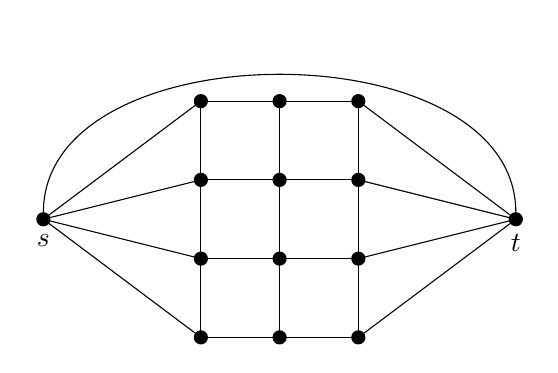
\begin{tikzpicture}[scale = 1]
					\tikzset{vertex/.style = {shape=circle,fill = black, draw, scale = 0.50}}
					\foreach \x in {0,1,2}{
						\foreach \y in {0,1,2,3}{
							\node[vertex] (\x\y) at (\x,\y) {};
					}}
					\draw (0,0) grid (2,3);
					\node[vertex] (s) at (-2, 1.5) {};
					\node[below=2pt] at (s) {$s$};
					\foreach \u in {00, 01, 02, 03}{
						\draw (s) -- (\u);
					}
					\node[vertex] (t) at (4, 1.5)  {};
					\node[below=2pt] at (t) {$t$};
					\foreach \w in {20, 21, 22, 23}{
						\draw (t) -- (\w);
					}
					\draw[out=90, in=90] (s) to (t);
				\end{tikzpicture}
			\end{center}
			
			\noindent \emph{Confirm or deny, with proof, whether Bullwinkle can always win if he employs a particular strategy for each move.}
			
			I suggest the following approach. 
			
			\begin{itemize}
				\item Show the graph has two disjoint spanning trees (spanning trees that share no edges). 
				\item Find an equivalent game that involves one player removing an edge of the graph and the other player drawing a multiedge instead of coloring edges. In other words, one player `colors' the edge by erasing it and the other player `colors' an edge by doubling it.
				\item Use theorems we have proved or will prove in class to argue your assertion. 
			\end{itemize}
			
			\begin{solution}
				
			\end{solution}
	\end{questions}
	
	
	\section{Invitation Madness}
	\qformat{\textbf{Sub-Adventure \thesection }\hfill}
	\begin{questions}
		
		\question You decide to use snail mail to send out invitations to a game night. Since you have never sent a piece of paper mail before in your life you start to worry that no one will receive the correct invitation. It occurs to you that there are more ways for everyone you invited to receive an invitation addressed to someone else than there are for everyone to receive the correct invitation.  This only serves to exacerbate your anxiety. You decide to calculate the number of ways that all of the invitations can be sent to the wrong person. 
		
		Determine the number $D_n$ of ways the $n$ invitations can be delivered to your $n$ friends so that no one gets the invitation actually intended for them.  
		
		Moreover, it is asked that you determine $D_n$ in a few ways: one way entails finding a recurrence relation for $D_n$, another entails a closed (albeit complicated) formula for $D_n$, and finally a fairly simple formula for $D_n$ obtained from the more complicated one. 
		
		\begin{parts}
			\part  Prove the recurrence $D_n = (n-1)D_{n-1} + (n-1)D_{n-2}$, for $n \geq 2$, with $D_0 = 1$ and $D_1 = 0$,
			
			\part   Derive, from the recurrence in sub-adventure 2(a), this recurrence $D_n = nD_{n-1} +(-1)^n$, for $n \geq 1$, with $D_0 = 1$.  
			
			\part Use the Principle of Inclusion-Exclusion to compute a closed formula for $D_n$.
			
			\part Noting that $e^x$ has a power series expansion $$e^x = 1 + x +\frac{x^2}{2!} + \frac{x^3}{3!} + \cdots + \frac{x^n}{n!} + \cdots,$$
			prove that $D_n$ is the nearest integer to $\frac{n!}{e}$; that is, 
			show that $$D_n = \left\lfloor \frac{n!}{e} + \frac{1}{2} \right\rfloor.$$
			(Now that's a nice and concise closed formula!)

		\begin{solution}
			\subsection*{Part (a):}
			\subsection*{Proof}
			We can prove the recurrence $D_n = (n-1)D_{n-1} + (n-1)D_{n-2}$ by using a combitorial argument. 

			First, we can choose any of the $n-1$ wrong invitations to send to the first person.  Then, we have two cases.  
			
			In the first case, we can send the invitation intended for the person who received the first person's invitation to the first person.  In this case, there are $D_{n-2}$ ways to count the remaining $n-2$ invitations.  
			
			In the second case, we can send the invitation intended for the person who received the first person's invitation to someone else.  In this case, there are $D_{n-1}$ ways to count the remaining $n-1$ invitations.  
			
			Since there are $n-1$ ways to choose which wrong invitation to send to the first person and since these cases are mutually exclusive, we have that $D_n = (n-1)D_{n-1} + (n-1)D_{n-2}$.

			\subsection*{Conclusion:}
			Thus, we have proved the recurrence $D_n = (n-1)D_{n-1} + (n-1)D_{n-2}$, for $n \geq 2$, with $D_0 = 1$ and $D_1 = 0$.


			\noindent\rule{\textwidth}{0.4pt}
			\subsection*{Part (b):}
			\subsection*{Proof}
			We can derive the recurrence $D_n = nD_{n-1} +(-1)^n$ from the recurrence in sub-adventure 2(a) by using induction.
			\subsection*{Base Case:}
			When $n=1$, we have $D_1 = 0$ and $1D_0 + (-1)^1 = 1(1) + (-1) = 0$.  Thus, the base case holds.

			\subsection*{Induction Step:}
			Assume that $D_k = kD_{k-1} +(-1)^k$ for all $k < n$.  We want to show that $D_n = nD_{n-1} +(-1)^n$.

			By the recurrence in sub-adventure 2(a), we know that $D_n = (n-1)D_{n-1} + (n-1)D_{n-2}$.  By the induction hypothesis, we have that $D_{n-1} = (n-1)D_{n-2} +(-1)^{n-1}$ and $D_{n-2} = (n-2)D_{n-3} +(-1)^{n-2}$.  
			
			After doing math, we can see that:
			\begin{align*}
				D_n &= (n-1)D_{n-1} + (n-1)D_{n-2} \\
				&= (n-1)((n-1)D_{n-2} +(-1)^{n-1}) + (n-1)((n-2)D_{n-3} +(-1)^{n-2}) \\
				&= (n-1)(n-1)D_{n-2} + (n-1)(-1)^{n-1} + (n-1)(n-2)D_{n-3} + (n-1)(-1)^{n-2} \\
				&= (n-1)(n-1)D_{n-2} + (n-1)(n-2)D_{n-3} + (n-1)(-1)^{n-1} + (n-1)(-1)^{n-2} \\
				&= (n-1)(n-1)D_{n-2} + (n-1)(n-2)D_{n-3} + (n-1)((-1)^{n-1} + (-1)^{n-2}) \\
				&= (n-1)(n-1)D_{n-2} + (n-1)(n-2)D_{n-3} + (n-1)(-1)^{n-2}((-1) + 1) \\
				&= (n-1)(n-1)D_{n-2} + (n-1)(n-2)D_{n-3} \\
				&= (n-1)((n-1)D_{n-2} + (n-2)D_{n-3}) \\
				&= (n-1)D_{n-1} \\
				&= nD_{n-1} +(-1)^n
			\end{align*}

			\subsection*{Conclusion:}

			Thus, we have shown that $D_n = nD_{n-1} +(-1)^n$.
			\noindent\rule{\textwidth}{0.4pt}

			\subsection*{Part (c):}
			Now our goal is to make a closed formula for $D_n$ by using the Principle of Inclusion-Exclusion.  
			
			We can do this by counting the number of ways to send the invitations so that at least one person gets the correct invitation and then subtracting this from the total number of ways to send the invitations.

			
			
		\end{solution}
			
		\end{parts}
	\end{questions}
	
	\section{An Optimization Problem}
	
	
	
	\qformat{\textbf{Sub-Adventure \thesection }\hfill}
	\begin{questions}
		\question 
		
		
		
		\noindent Let $H$ denote an arbitrary graph. The distance between vertices in $H$ is the length of the shortest path that has those vertices as its endpoints.  Denote by $d_{\mathrm{max}}(H)$ the maximum distance among all pairs of vertices of $H$.
		Note that $\Delta(H)$ denotes the maximum degree among all vertices of $H$.\\
		
		
		\noindent Define the function $N(d,k)$ to be the maximum number of vertices among all graphs $H$ with $d_{\mathrm{max}}(H) = d$ and $\Delta(H) = k$.\\
		
		\begin{minipage}{.5\linewidth}
			\begin{parts}
				\part \emph{Determine $N(n,2)$.}
				
				\part\emph{Determine $N(2,3)$.}
				
				\part \emph{Verify that the graph $G$ drawn to the right has $d_{\mathrm{max}}(G) =2$.}
				
				\part Give bounds for $N(2,4)$. \emph{Bonus: Determine $N(2,4)$.}
			\end{parts}
			
		\end{minipage}
		\begin{minipage}{.5\linewidth}
			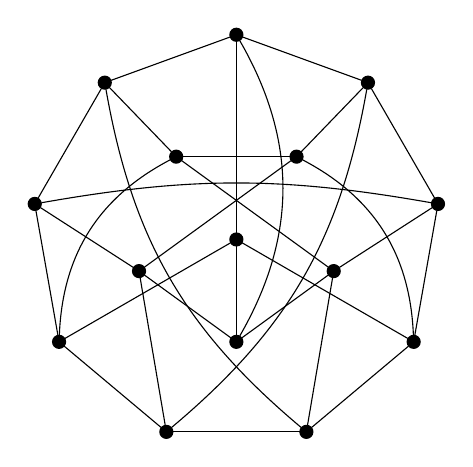
\begin{tikzpicture}[scale = 1]
				\tikzset{vertex/.style = {shape=circle,fill = black, draw, scale = 0.50}}
				\newcommand\rad{1.3}
				\newcommand\Rad{2.6}
				\foreach \a/\t/\r in {14/0/0, 
					15/-90/\rad, 13/-18/\rad, 12/54/\rad, 11/126/\rad, 10/198/\rad,
					1/90/\Rad, 2/50/\Rad, 3/10/\Rad, 4/-30/\Rad, 5/-70/\Rad, 6/-110/\Rad, 7/210/\Rad, 8/-190/\Rad, 9/-230/\Rad}{
					\node[vertex] (\a) at (\t:\r) {};
				}
				\draw (1) to (2);
				\draw (1) to (9);
				\draw (1) to (14);
				\draw[bend left] (1) to (15);
				\draw (2) to (3);
				\draw (2) to (12);
				\draw[bend left=20] (2) to (6);
				\draw (3) to (4);
				\draw[bend right=10] (3) to (8);
				\draw (3) to (13);
				\draw (4) to (5);
				\draw[bend right] (4) to (12);
				\draw (4) to (14);
				\draw (5) to (6);
				\draw[bend left=20] (5) to (9);
				\draw (5) to (13);
				\draw (6) to (7);
				\draw (6) to (10);
				\draw (7) to (8);
				\draw[bend left] (7) to (11);
				\draw (7) to (14);
				\draw (8) to (9);
				\draw (8) to (10);
				\draw (9) to (11);
				\draw (10) to (12);
				\draw (10) to (15);
				\draw (11) to (12);
				\draw (11) to (13);
				\draw (13) to (15);
				\draw (14) to (15);
			\end{tikzpicture}
			
			
		\end{minipage}
		
		\begin{solution}
			
		\end{solution}
		
		
	\end{questions}
	
	
	
		\section{Stirling Numbers}
	\qformat{\textbf{Sub-Adventure \thesection.\thequestion }\hfill}
	\begin{questions}
		
		\question  	Let $\mathcal{N}$ denote the set of all possible ways to place $s$ labeled balls into $t$ labeled boxes so that no box is empty. Recall from your midterm that $|\mathcal{N}| = t!\stirling{s}{t}$. Use the recurrence $\stirling{n}{k} = k \stirling{n-1}{k} + \stirling{n-1}{k-1}$ to create a generating function for the Stirling numbers by following the steps below.
		
		\begin{parts}
			\part  Let $k$ be a fixed but arbitrary number and set 
			
			\[f_k(x) = \sum_{n=k}^\infty \stirling{n}{k}x^n\]
			
			Explain why the sum does not start when $n=0$ and show $kxf_{k}(x)+x f_{k-1}(x) = f_{k}(x)$.
			
			\part Solve for $f_k(x)$ in the equation from part (a) and then iterate the resulting recurrence to obtain
			
			\[f_k(x) = x^k \prod_{r=1}^{k} \frac{1}{(1-rx)}\]


			\part Now calcluate $|\mathcal{N}|$ by using the Principle of Inclusion--Exclusion. Use your result to conclude that

			\[\stirling{s}{t} = \sum_{k=0}^t \frac{(-1)^k (t-k)^s}{k! (t-k)!}\]
			
			
			
		
			
		\end{parts}

		\begin{solution}
			
		\end{solution}
	\end{questions}


	\section{Flocks}
	
	
	\subsection*{Queens}
	
	\qformat{\textbf{Sub-Adventure \thesection.\thequestion }\hfill}
	\begin{questions}
		\question 
		{\bf Queens.}  
		Let $n$ and $q$ be positive integers with $q \leq n$.  
		Define an $(n,q)$-flock to be a flock on $n$ vertices with exactly $q$ queens.
		In this sub-adventure, you will determine all possible values of $n$ and $q$ for which there exists an $(n,q)$-flock.
		Specifically, please prove the following theorem.\\
		
		\begin{theorem}There exists an $(n,q)$-flock for all positive integers $n$ and $q$ with $n \geq q \geq 1$, except for 
			$q = 2$ and arbitrary $n$, and $n = q = 4$.
		\end{theorem}
		
		\noindent I suggest that you use the Principle of Mathematical Induction and the following lemmas (which I ask that you prove as well).\\
		
		\begin{lemma}
			There exists a $(1,1)$-flock.
		\end{lemma}
		
		
		\begin{lemma}
			There does not exist a $(4,4)$-flock.
		\end{lemma}
		
		
		\begin{lemma}
			There is a $(6,6)$-flock.
		\end{lemma}
		
		
		\begin{lemma}
			If there exists an $(k,k)$-flock, then there exists an $(k+2, k+2)$-flock, where $k$ is a positive integer.
		\end{lemma}
		
		
		\begin{lemma}
			For every positive integer $n$ except $2$ and $4$, there exists an $(n,n)$-flock.
		\end{lemma}
		
		
		
		\begin{solution}
			
		\end{solution}
		
	
		
	
	\end{questions}
	
	
\end{document}
